%Autor: Simon Walker
%Version: 1.0
%Datum: 09.12.2019
%Lizenz: CC BY-NC-SA

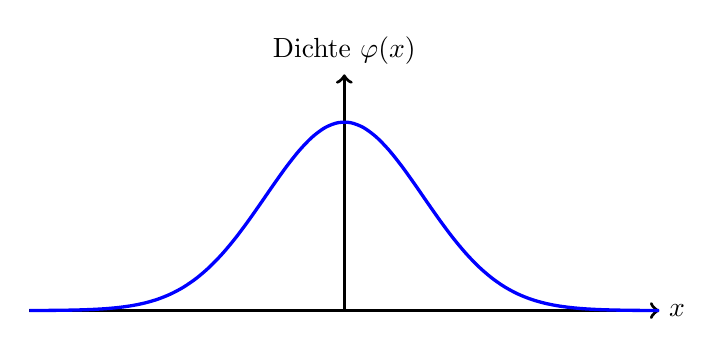
\begin{tikzpicture}[xscale=1, yscale=6]
	
	%Achse
	\draw[very thick, ->] (-4, 0) -- (4, 0);
	\draw[very thick, ->] (0, 0) -- (0, 0.5);
	\node[right] at (4, 0) {$x$};
	\node[above] at (0, 0.5) {Dichte $\varphi(x)$};
	
	\draw[blue, very thick, smooth]
	plot[smooth, samples=50, variable=\x, domain=-4:4]
		(\x, {0.3989*exp(-((\x)^2)/2)});

\end{tikzpicture}
